%!TEX root = ../crimson_throne_book_main.tex
% 2016-01-23
\section{12 Arodus 4708}

In the traditional Burn Run young aspiring Sun Clan warriors have to stay ahead of a wildfire. Krojun advises the 'tshamek' to do the same in the auroch run, because {\itshape``once those beasts catch up, you're lost}'', he claims. Sjo has prepared by removing his full plate and Quint and Balian get ready by casting a few spells. Quint enhances everyone's general performance with {\itshape heroism} and his own speed with  {\itshape expeditious retreat} . Balian whips out his  {\itshape longstrider} to be a bit faster. The three companions and their Shoanti challenger are waiting at the mouth of a one mile long rift through the Kallow hills. Their goal is a standing stone at the end of the canyon; they have to reach the top safely before being overrun by the aurochs. Krojun's own companions have left early in the morning to locate the great herd and drive it towards the rift. A big cloud of dust over the hills heralds their arrival. When the proud animals finally pop into view, the race starts. Sjo calls down his {\itshape blessing of fervor} to hasten himself and Balian. Krojun uses his barbarian speed and immediately breaks into a sprint. Still, the companions' magically enchanced speed sends them all in front of him. Quint decides to play the game for maximum effect and waits for the mighty barbarian, trying to hang around his position during the entire race. In the meantime Balian chooses to get the most out of his magical velocity and runs as far ahead as he can, while Sjo attempts to slow the herd by throwing a  {\itshape fireball} in front of it. The panic slows the animals only for a second, before sending them into a wild bolt down the rift. Now the stampede has truly begun! Sjo runs off again and renews his {\itshape blessing of fervor} , for its powerful pace lasts only a few dozen heartbeats. Now he can close in on Balian again, who successfully jumps over a wide pit that spans the floor of the canyon from left to right. Sjo summons his fiery wings to cover the distance. Behind him Krojun has little trouble leaping over the gaping hole, but Quint does not make it to the far side and loses a handful of precious seconds to crawl out. Still, the bard is not worried, his superior  {\itshape expeditous retreat} speed easily allows him to play a game of catch and release with Krojun. He catches up again, bluffs his face into a {\itshape``wheh, that was exciting}'' look and continues the race. Sjo has to renew his hastening magic twice more, making sure to cover Balian in the spell as well. The two companions have a nice lead on the two other runners, until they have to slow their advance to a hustle - continuing to sprint would only result in exhaustion. This allows Krojun and Quint to close the gap between them. The trampling herd follows hot on their heels. Finally the standing stone pops into view. By now Quint and Krojun have overtaken Balian, and the bard bolts ahead to reach the finish first. Sjo is the second to arrive, summoning his wings once more to reach the top of the stone. Krojun and Balian arrive seconds later, just in front of the thundering herd.\hyperref[fig:The-auroch-run-vs-Shoanti-Krojun-586163164]{ From the top the finishers witness the impressive wild herd storm past. } When the dust settles the burn riders and the Skull Clan members arrive, cheering at the runners' success. Krojun smiles broadly at Sjo and his friends. While he doesn't yet see the companions as true  {\itshape nalharest} , his gaze glazes with respect. \\

\begin{figure}[h]
	\centering
	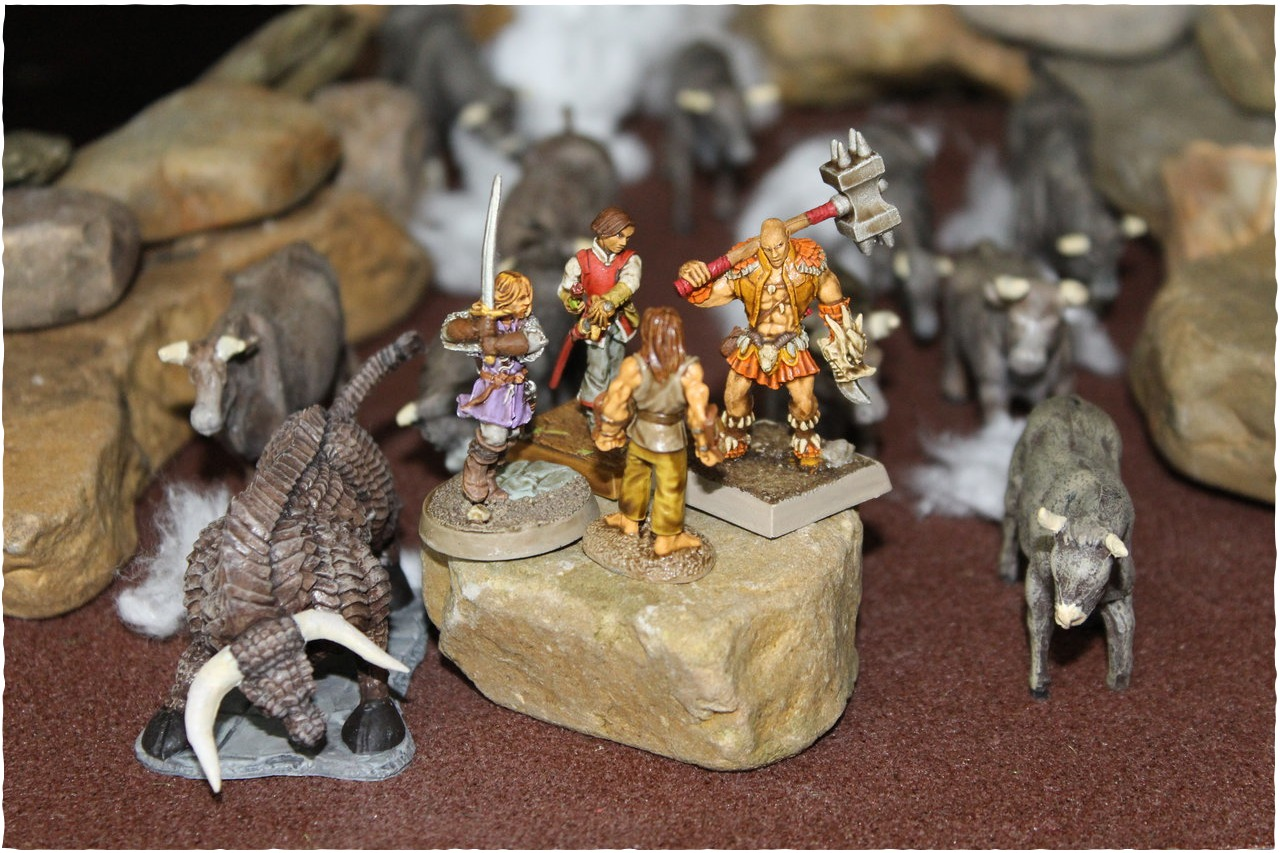
\includegraphics[width=0.4\textwidth]{images/The-auroch-run-vs-Shoanti-Krojun-586163164_mod.jpg}
	\caption{The auroch run vs. Shoanti Krojun}
	\label{fig:The-auroch-run-vs-Shoanti-Krojun-586163164}
\end{figure}

The companions spend the rest of the day basking in the glory of their victory. They learn that the Sun Clan has sent out many riders to gather all Shoanti tribes in the shadow of the Great Flame, an immense rock pinnacle in the heart of the Cinderlands. Krojun continues his efforts to enlist new warriors for this army, while Sjo and Quint try to sew doubt in the minds of the Skull Clan members, telling them about the might of Korvosa's new ruler.\\

In the evening Thousand Bones informs his guests that he has prepared the teleport ritual. He will send the party to the Hold of Belkzen tomorrow.\\

\section{13 Arodus 4708}

The next morning Thousand Bones leads the companions deeper into the Kallow Hills, to a rocky hilltop with a circle of menhirs. The majestic stones have been decorated with intricate patterns. A large flat stone lies in the center of the circle. Thousand Bones tells the party to stand on it. {\itshape``Remember, you need a token to get into the city}'', he says, before bursting into a chant. He squeezes two small bird skulls to dust and sends the pulverized bone over the standing stones, which start to glow with magic. A big flash ensues and the heroes feel like their stomachs are being turned inside out and their eyes are pushed deep into their sockets. The next moment they have arrived in a desolate plain. The landscape definitely resembles the Cinderlands: dusty and dry, full of rocks and a handful of shriveled bushes and dead trees. The only feature on the horizon is an elevation to the northeast, so the party decides to head that way.\\

The sun seems even hotter here than it did in the Cinderlands. Fortunately Sjo's magic can provide an endless stream of refreshing water, while his magic keeps the companions from suffering any ill effect from the heat. A few hours into the afternoon Quint hears a feeble rumble and feels the earth tremble ever so slightly. Before his friends can react, the ground tears open and four bulettes burst through the sand. These mighty monsters are known as land shark, but are at least ten times as deadly as their marine counterparts. Balian suffers the frontal assault of the biggest and meanest specimen and Sjo struggles to keep the ranger on his feet with his healing magic. A smaller bulette leaps through the air to Quint, who has taken a few steps back to cast {\itshape haste} on his friends. A  {\itshape mirror image} saves him from the worst attacks, while Balian and Puk exchange blows with the other three beasts. They barely manage to take out the leader, kept alive by the grace of Sjo's  {\itshape cure critical wounds} . Quint turns the tide of the battle by taking out another bulette with his  {\itshape cacophonous call} , sending the monster back into the earth. While his friends take care of a third land shark, the bard successfully repeats his magic on the smallest beast, which flees the scene as well. He thanks the gods that the creatures did not resist his spells, realizing that his friends might not have survived if they had. While the companions nurse their wounds, they notice a cloud of dust closing in. Balian squeezes and makes out the shapes of running wargs: big, bad wolves with riders on their backs.\\

